\documentclass{article}

\usepackage{graphicx}
\usepackage{tikz}
\usepackage{tikzsymbols}
\usetikzlibrary{calc,patterns,shapes.geometric}
\pagestyle{empty}
\usepackage[margin=0pt]{geometry}
\geometry{papersize={14in,12in}}

\def\centerarc[#1](#2)(#3:#4:#5){\draw[#1] ($(#2)+({#5*cos(#3)},{#5*sin(#3)})$) arc (#3:#4:#5);}

\begin{document}
	\begin{figure}
		\centering
		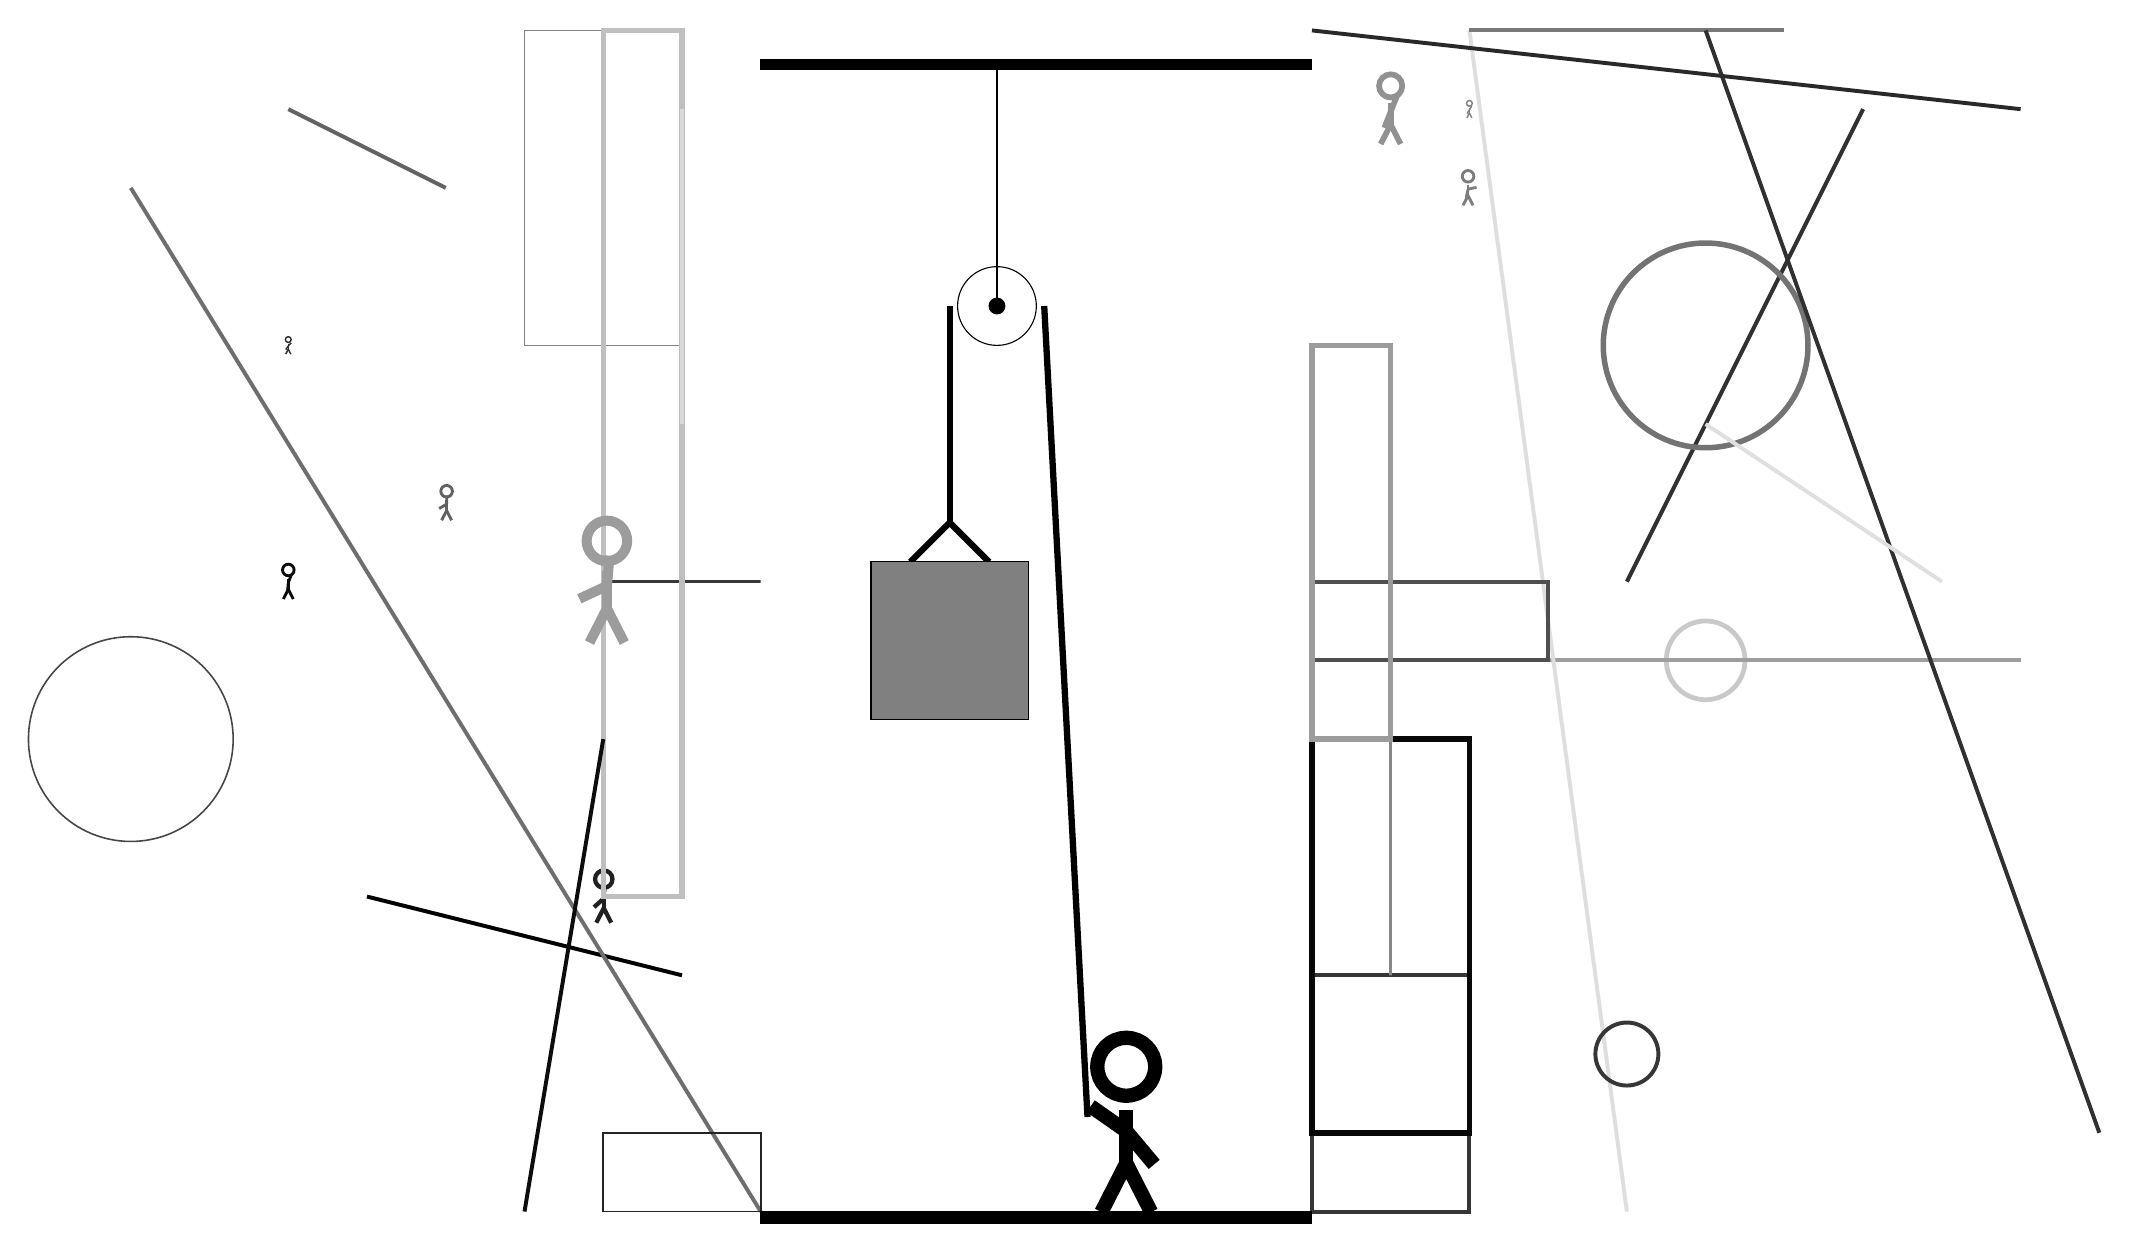
\begin{tikzpicture}
			%%%%% START %%%%%
			
			\draw[fill=black] (-2, 11.5) rectangle (5, 11.625);
			
			\draw (1, 8.5) circle (0.5);
			\draw[fill=black] (1, 8.5) circle (0.1);
			\draw (1, 11.5) -- (1, 8.5);
			
			\draw [line width=0.6mm, color=black!21](10, 4) circle (0.5);
			
			\node[line width=0.6mm, color=black!96] at (-8, 5) {\Strichmaxerl[2][85][70]};
			\draw[line width=0.5mm, color=black!79] (5, 0) rectangle (7, -3);
			\node[line width=0.6mm, color=black!83] at (-8, 8) {\Strichmaxerl[1][55][47]};
			
			\node[line width=0.4mm, color=black!87] at (-4, 1) {\Strichmaxerl[3][42][87]};
			\draw[line width=0.5mm, color=black!81](9, 5) -- (12, 11);
			
			\draw[line width=0.2mm, color=black!49] (-3, 8) rectangle (-5, 12);
			
			\draw[line width=0.5mm, color=black!38](5, 4) -- (14, 4);
			\node[line width=0.5mm, color=black!43] at (6, 11) {\Strichmaxerl[4][69][68]};
			\draw [line width=0.7mm, color=black!55](10, 8) circle (1.3);
			\draw [line width=0.2mm, color=black!73](-10, 3) circle (1.3);
			
			\draw[line width=0.5mm, color=black!13](9, -3) -- (7, 12);
			\node[line width=0.3mm, color=black!50] at (7, 11) {\Strichmaxerl[1][59][57]};
			\draw[line width=0.3mm, color=black!78] (-4, 5) rectangle (-2, 5);
			\draw[line width=0.7mm, color=black!25] (-4, 1) rectangle (-3, 12);
			\draw[line width=0.5mm, color=black!53](7, 12) -- (11, 12);
			
			\node[line width=0.2mm, color=black!39] at (-4, 5) {\Strichmaxerl[7][25][85]};
			\draw[line width=0.5mm, color=black!100](-3, 0) -- (-7, 1);
			\draw[line width=0.5mm, color=black!69] (5, 5) rectangle (8, 4);
			
			\draw[line width=0.5mm, color=black!61](-6, 10) -- (-8, 11);
			\draw[line width=0.5mm, color=black!81](10, 12) -- (15, -2);
			\draw[line width=0.5mm, color=black!57](-2, -3) -- (-10, 10);
			\draw[line width=0.7mm, color=black!97] (5, -2) rectangle (7, 3);
			\draw[line width=0.4mm, color=black!47] (6, 0) rectangle (6, 6);
			\node[line width=0.4mm, color=black!62] at (-6, 6) {\Strichmaxerl[2][31][89]};
			\draw[line width=0.5mm, color=black!95](-4, 3) -- (-5, -3);
			\node[line width=0.4mm, color=black!51] at (7, 10) {\Strichmaxerl[2][78][12]};
			\draw[line width=0.5mm, color=black!84](5, 12) -- (14, 11);
			\draw [line width=0.5mm, color=black!79](9, -1) circle (0.4);
			\draw[line width=0.5mm, color=black!15] (-3, 7) rectangle (-3, 11);
			\draw[line width=0.7mm, color=black!39] (6, 8) rectangle (5, 3);
			\draw[line width=0.2mm, color=black!86] (-4, -2) rectangle (-2, -3);
			\draw[line width=0.5mm, color=black!12](10, 7) -- (13, 5);
			
			\draw[line width=0.8mm] (-0.1, 5.25) -- (0.4, 5.75) -- (0.9, 5.25);
			\draw[fill=black!50] (-0.6, 5.25) rectangle (1.4, 3.25);
			
			\draw[line width=0.8mm] (0.4, 8.5) -- (0.4, 5.75);
			\centerarc[line width=0.8mm](1, 8.5)(0:180:0.6);
			\draw[line width=0.8mm](1.6, 8.5) -- (2.15, -1.8);
			
			\node at (2.6, -1.9) {\Strichmaxerl[10][-35][-50]};
			
			\draw[fill=black] (-2, -3) rectangle (5, -3.15);
			
			%%%%% END %%%%%
		\end{tikzpicture}
	\end{figure}	
\end{document}